\section{The quadratic relation in general}

    In this section we show that for any character $\chi=\chi_0\otimes\ldots\otimes\chi_n$ of $T(\cO)\subset\GL_{n+1}(F)$ and $s\in S_{\chi,\aff}$, the proof of the quadratic relation for $\varphi_s=q^{(1-l(s))/2}[IsI]_{\check{\chi}}$ can be deduced from the particular case proven in the previous section. Let $\Phi$ be the root system for $\GL_{n+1}$ with simple roots $\Pi=\{\alpha_1,\ldots,\alpha_n\}$. For each $w\in\tilde{W}$, let 
    $$\widetilde{\Delta}(w)=\{\text{hyperplanes }P\ |\ P\text{ separates }\mathcal{D}_0\text{ and }w\mathcal{D}_0\}.$$
    Recall from Iwahori-Matsumoto that $l(w)=|\widetilde{\Delta}(w)|$ for all $w\in\tilde{W}$.

    \begin{lemma}\label{lem_w1}
        Let $\alpha=\sum_{k=i}^{j}\alpha_k\in\Phi^+$ for some $i\leq j$. Then
        \begin{align*}
            \widetilde{\Delta}(w_\alpha(1))&=\{P_{\beta,0}\ |\ \beta\in\Phi^+\cap w_\alpha^{-1}\Phi^-\}\\
            %=\{P_{\alpha,0}\}\cup\{P_{\beta,0}:\beta\in\Phi^+,\langle\beta,\calpha\rangle=1\text{ and }\alpha-\beta\in\Phi^+\}\\
            &=\{P_{\alpha_i,0},P_{\alpha_i+\alpha_{i+1},0},\ldots,P_{\alpha,0},\ldots,P_{\alpha_{j-1}+\alpha_j,0},P_{\alpha_j,0}\}.
        \end{align*}
    \end{lemma}

    \begin{proof}
        Let $x\in\mathcal{D}_0$ and let $\beta\in\Phi^+$. Then
        \begin{equation*}
            \langle\beta,w_\alpha(1)(x)\rangle=\langle\beta,x\rangle-\langle\alpha,x\rangle\langle\beta,\calpha\rangle=\langle w_\alpha(\beta),x\rangle\in
            \begin{cases}
                (0,1) &\text{ if } w_\alpha(\beta)\in\Phi^+,\\
                (-1,0) &\text{ if } w_\alpha(\beta)\in\Phi^-.
            \end{cases}
        \end{equation*}
        Hence, $P\in\widetilde{\Delta}(w)$ if and only if $P=P_{\beta,0}$ for some $\beta\in\Phi^+\cap w_\alpha^{-1}\Phi^{-1}$. Since $w_\alpha(\beta)=\beta-\langle\beta,\calpha\rangle\alpha$, it follows that $\beta\in\Phi^+\cap w_\alpha^{-1}\Phi^-$ if and only if $\beta=\alpha$ or $\langle\beta,\calpha\rangle=1$ and $\alpha-\beta\in\Phi^+$.
        
        If $\alpha=\alpha_i+\cdots+\alpha_j$ for some $j\geq i$, then a standard calculation shows that $\beta\in\Phi^+$ satisfies the above conditions if and only if $\beta=\alpha_i+\cdots+\alpha_k$ for some $k\leq j$ or $\beta=\alpha_k+\cdots+\alpha_j$ for some $k\geq i$. This concludes the proof.
    \end{proof}

    \begin{lemma}\label{lem_wvarpi}
        Let $\alpha=\sum_{k=i}^{j}\alpha_k\in\Phi^+$ for some $i\leq j$. Then
        \begin{align*}
            \widetilde{\Delta}(w_\alpha(\varpi^{-1}))&=\{P_{\alpha_1+\cdots+\alpha_{i-1},0},\ldots,P_{\alpha_{i-1},0},P_{\alpha_{j+1},0},\ldots,P_{\alpha_{j+1}+\cdots+\alpha_{n},0}\}\\
            %=\{P_{\alpha,0}\}\cup\{P_{\beta,0}:\beta\in\Phi^+,\langle\beta,\calpha\rangle=1\text{ and }\alpha-\beta\in\Phi^+\}\\
            &\cup\{P_{\alpha_1+\cdots+\alpha_j,1},\ldots,P_{\alpha_i+\cdots+\alpha_{j},1},\ldots,P_{\alpha_i+\cdots+\alpha_n,1}\}.
        \end{align*}
    \end{lemma}

    \begin{proof}
        As in the previous proof, let $x\in\mathcal{D}_0$ and let $\beta\in\Phi^+$. Then,
        \begin{align*}
            \langle\beta,w_\alpha(\varpi^{-1})(x)\rangle=\langle\beta,x\rangle-\langle\alpha,x\rangle\langle\beta,\calpha\rangle+\langle\beta,\calpha\rangle=\langle w_\alpha(\beta),x\rangle+\langle\beta,\calpha\rangle\\
            \in
            \begin{cases}
                (1,2) &\text{ if } \beta=\alpha \text{, or } \langle\beta,\calpha\rangle=1 \text{ and } w_\alpha(\beta)\in\Phi^+,\\
                (0,1) &\text{ if } \langle\beta,\calpha\rangle=0 \text{, or }\langle\beta,\calpha\rangle=1 \text{ and }w_\alpha(\beta)\in\Phi^-,\\
                (-1,0) &\text{ if } \langle\beta,\calpha\rangle=-1.
            \end{cases}
        \end{align*}
    
        Thus,
        \begin{equation*}
            \widetilde{\Delta}(w_\alpha(\varpi^{-1}))=\{P_{\alpha,1}\}\cup\{P_{\beta,1}\ |\ \beta\in\Phi^+,\langle\beta,\calpha\rangle=1 \text{ and }w_\alpha(\beta)\in\Phi^+\}\cup\{P_{\beta,0}\ |\ \beta\in\Phi^+\text{ and }\langle\beta,\calpha\rangle=-1\}.
        \end{equation*}
        If $\alpha=\alpha_i+\cdots+\alpha_j$, then further calculations show that $\beta\in\Phi^+$ satisfies $\langle\beta,\calpha\rangle=1$ with $w_\alpha(\beta)=\beta-\alpha\in\Phi^+$ if and only if $\beta=\alpha_k+\cdots+\alpha_j$ for some $k<i$ or $\beta=\alpha_i+\cdots+\alpha_k$ for some $k>j$. Similarly, one can show that $\beta\in\Phi^+$ satisfies $\langle\beta,\calpha\rangle=-1$ if and only if $\beta=\alpha_k+\cdots+\alpha_{i-1}$ for some $k\leq i-1$ or $\beta=\alpha_{j+1}+\cdots+\alpha_k$ for some $k\geq j+1$.
    \end{proof}


    \begin{cor}\label{cor_lengthsum}
        For any $\alpha\in\Phi^+$, we have that 
        $$l(w_\alpha(1))+l(w_\alpha(\varpi^{-1}))=\sum_{\beta\in\Phi^+}|\langle\beta,\calpha\rangle|=2n$$
    \end{cor}
    \begin{proof}
        The first equality is an immediate consequence of $l(w)=\widetilde{\Delta}(w)$ together with Lemmas \ref{lem_w1} and \ref{lem_wvarpi}. Indeed, if $\langle\beta,\calpha\rangle=0$ then no hyperplane arising from $\beta$ lies in $\widetilde{\Delta}(w_\alpha(1))\cup\widetilde{\Delta}(w_\alpha(\varpi^{-1}))$; if $\langle\beta,\calpha\rangle=\pm1$, then exactly one plane arising from $\beta$ lies $\widetilde{\Delta}(w_\alpha(1))\cup\widetilde{\Delta}(w_\alpha(\varpi^{-1}))$; finally, $P_{\alpha,0}\in \widetilde{\Delta}(w_\alpha(1))$ and $P_{\alpha,1}\in \widetilde{\Delta}(w_\alpha(\varpi^{-1}))$.

        The second part of the lemma is a direct computation: if $\alpha=\alpha_i\cdots\alpha_j$, then there are 
        \begin{itemize}
            \item $j$ roots in $\Phi^+$ of the form $\alpha_k+\cdots+\alpha_j$ for $k\leq j$,
            \item $n+1-i$ roots in $\Phi^+$ of the form $\alpha_i+\cdots+\alpha_k$ for $k\geq i$,
            \item $i-1$ roots in $\Phi^+$ of the form $\alpha_k+\cdots+\alpha_{i-1}$ for $k\leq i-1$,
            \item $n+1-(j+1)$ roots in $\Phi^+$ of the form $\alpha_{j+1}+\cdots+\alpha_k$ for $k\geq j+1$.
        \end{itemize}
        Giving a total of $2n$ roots, each of which contributes once towards $\sum_{\beta\in\Phi^+}|\langle\beta,\calpha\rangle|$, as desired.
    \end{proof}

    \subsection{The diagram associated to a character}
    Having established the preliminary lemmas, we now consider a depth zero character $\chi=\chi_0\otimes\cdots\otimes\chi_n$ of $T(\cO)\subset\GL_{n+1}(F)$, where each $\chi_i$ is a depth-zero character of $\cO^\times$. The character $\chi$ induces a partition $\mathcal{P}_\chi$ of the set $\{0,1,\ldots,n\}$ according to which two elements $i,j\in\{0,1,\ldots,n\}$ are related if and only if $\chi_i=\chi_j$ as characters of $\cO^\times$. Denote by $\mathfrak{D}_{n}$ the affine Dynkin diagram of type $A_n$ (a regular polygon whose vertices are labelled $\alpha_0,\alpha_1,\ldots,\alpha_n$ counterclockwise) and whose edges have been labelled from $0$ to $n$ according to the correspondence 
    \begin{align*}
        \{0,1,\ldots,n\}&\longrightarrow\{\text{edges of }\mathfrak{D}_n\}\\
        k&\longmapsto
        \begin{cases}
            \{\alpha_k,\alpha_{k+1}\} &\text{ if }k\neq n,\\
            \{\alpha_n,\alpha_0\} &\text{ if }k=n.
        \end{cases}.
    \end{align*}
    In addition, we distinguish the vertex $\alpha_0$.

    \begin{definition}
        Let $\chi$ be a depth-zero character of $T(\cO)\subset\GL_{n+1}(F)$ giving rise to a partition $\mathcal{P}_\chi$ of $\{0,1,\ldots,n\}$ of size $r$. Then the \textit{Dynkin diagram $\mathfrak{D}_\chi$ associated to} $\chi$ is the Dynkin diagram $\mathfrak{D}_n$ whose edges have been colored in $r$ distinct colors according to the partition $\mathcal{P}_\chi$.        
    \end{definition}
    \begin{example}
        In the previous section we considered the family of characters $\chi=\chi_0\otimes\cdots\otimes\chi_n$ such that $\chi_0=\chi_n$ and all the remaining characters are distinct. Then $\mathcal{P}_\chi=\{\{0,n\},\{1\},\ldots,\{n-1\}\}$ has size $n$, and Figure \ref{fig_diagn4} shows the diagram $\mathfrak{D}_\chi$ for $n=4$.
        \begin{figure}[h]
            \begin{center}
                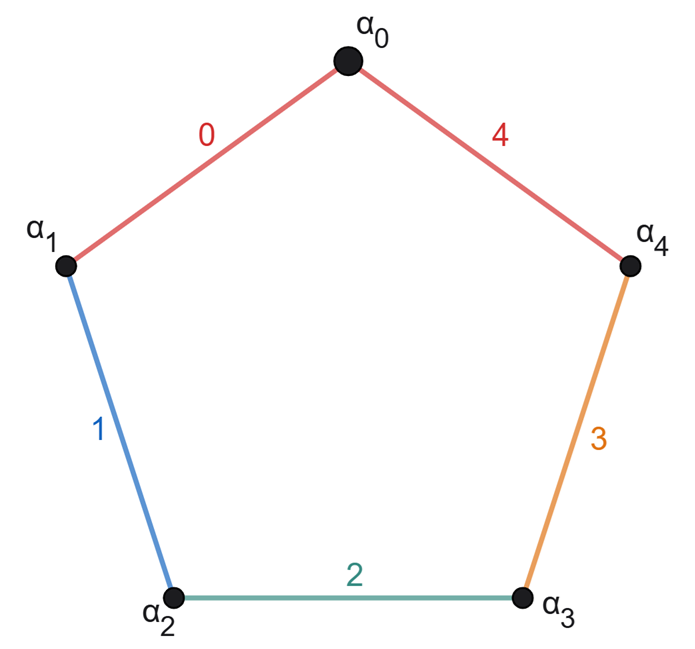
\includegraphics[scale=0.6]{dynkin_diagram_labels.png}
                \caption{Diagram for $\mathcal{P}_\chi=\{\{0,4\},\{1\},\{2\},\{3\}\}$}
                \label{fig_diagn4}
            \end{center}
        \end{figure}
    \end{example}


    The diagram of a character defined above is useful because it will allow us to determine $S_{\chi,\aff}$ easily. The first step towards this goal is to associate elements of $\widetilde{W}_\chi$ to paths between edges in the diagram.

    \begin{definition}
        Let $\mathfrak{D}_\chi$ be the diagram associated to $\chi$ and let $i,j\in\{0,1,\ldots,n\}$ be two \textit{distinct} edges, and we assume that $i<j$. Let 
        $$\alpha_{i,j}=\alpha_{i+1}+\cdots+\alpha_{j-1}+\alpha_j\in\Phi^+$$
        be the positive root associated to the pair $(i,j)$. Let $T_{i,j,1}$, (resp. $T_{i,j,0}$) be the two trails in $\mathfrak{D}_\chi$ from $i$ to $j$ avoiding (resp. passing through) the distinguished edge $e=\{0,n\}$. Then the associated reflection $w(T_{i,j,k})$ to the path $T_{i,j,k}$ is
        \begin{equation*}
            w(T_{i,j,k})=
            \begin{cases}
                w_{\alpha_{i,j}}(1) &\text{ if } k=1,\\
                w_{\alpha_{i,j}}(\varpi^{-1}) &\text{ if } k=0.
            \end{cases}
        \end{equation*}
    \end{definition}

    \begin{lemma}
        For any path $T_{i,j,k}$, we have that 
        $$l(w(T_{i,j,k}))=2l(T_{i,j,k})-1,$$
        where the length of a trail is the number of edges on the trail.
    \end{lemma}
    \begin{proof}
        Assume without loss of generality that $i<j$. 
        If $k=0$, then $l(T_{i,j,0})=j-i$, while Lemma \ref{lem_w1} shows that $l(w_{\alpha_{i,j}}(1))=2(j-i)+1$. If $k=1$, we may use Corollary \ref{cor_lengthsum} to obtain
        $$l(w_{\alpha_{i,j}}(\varpi^{-1}))=2n-l(w_{\alpha_{i,j}}(1))=2n-2l(T_{i,j,0})+1=2(n+1-l(T_{i,j,0}))-1=2l(T_{i,j,1})-1,$$
        and this concludes the lemma.
    \end{proof}

    \begin{proposition}
        Let $\chi$ be a depth-zero character of $T(\cO)$ and let $\mathfrak{D}_\chi$ be the associated diagram induced by the partition $\mathcal{P}_\chi=\{A_1,\ldots,A_r\}$ of its vertices. For each set $k\in\{1,\ldots,r\}$, write $A_k=\{a_{k,1}<\cdots<a_{k,m_k}\}$ and let $\{T_{k,i}\ |\ i=1,\ldots,m_k\}$ be all the paths joining each consecutive pair of vertices in $A_k$. Then
        \begin{equation*}
            S_{\chi,\aff}=\bigcup_{k=1}^r \{w(T_{k,1}),\ldots,w(T_{k,m_k})\}.
        \end{equation*}
    \end{proposition}

    \begin{proof}
        Firstly, we note that if $\mathcal{P}_\chi=\{A_1,\ldots,A_r\}$, which each $A_k$ of size $m_k$, then 
        $$\widetilde{W}_\chi\cong \widetilde{W}_{\chi^{(1)}}\times\cdots\times\widetilde{W}_{\chi^{(r)}},$$
        where $\chi^{(k)}=\chi_{a_{k,1}}\otimes\cdots\otimes\chi_{a_{k,m_k}}$ is the depth-zero character of $\GL_{m_k}$, and $\widetilde{W}_{\chi^{(k)}}$ is viewed as a subgroup of $\widetilde{W}_{\chi}$ in the obvious way. Each $\widetilde{W}_{\chi^{(k)}}$ is an extended Weyl group in its own right, and if we let $S_{\chi,\aff,k}$ be the set of simple reflections of $\widetilde{W}_{\chi^{(k)}}$ viewed as a subgroup of $\widetilde{W}_{\chi}$, then 
        $$S_{\chi,\aff}=\bigcup_{k=1}^r S_{\chi,\aff,k}.$$
        It therefore suffices to show that 
        $$S_{\chi,\aff,k}=\{w(T_{k,1}),\ldots,w(T_{k,m_k})\}.$$
        \textcolor{red}{still remains to prove this, which is definitely expected to be true!}
    \end{proof}
        
    \subsection{The induced homomorphism on Hecke algebras}

    Having established a way to easily determine $S_{\chi,\aff}$ from the depth-zero character $\chi$, we now fix some $s\in S_{\chi,\aff}$ and deduce the quadratic relation for $\varphi_s=q^{(1-l(s)/2)}[IsI]_{\check{\chi}}$ using the results in the previous section. To do this, we first note that $s$ corresponds to some trail $T_s$ on $\mathfrak{D}_\chi$ of length $l(T_s)=(l(s)+1)/2$. 

    We also need to consider the element 
    \begin{equation*}
        \rho_n:=
        \begin{pmatrix}
            &1&& \\
            &&\ddots& \\
            &&&1 \\
            -\varpi&&& 
        \end{pmatrix},
    \end{equation*}
    which is the generator of the alcove stabilizer $\Omega$.

    \begin{lemma}
        The action of $\rho_n$ on the space of depth-zero characters of $T(\cO)$ induces an action on the diagrams given by a counterclockwise rotation of $2\pi/n$ radians. In other words, 
        $$\mathfrak{text}$$
    \end{lemma}
